% =====================================================================
% Conference paper in ieeeconf format, targeting ECC. 6-page limit.
%
% FRAMING (settled): the paper's object is the LIMIT CYCLE of fixed-step
% and accelerated SPIN tuning. The triple point is the tool that locates
% the cycle's center; the regularized index is the tool that makes the
% analysis well posed. Neither appears in the title.
%
% Numbers policy: all from verified follow-up runs. TODO-REGEN entries
% need regeneration before submission; TODO marks editorial placeholders.
% =====================================================================
\documentclass[letterpaper, 10pt, conference, twocolumn]{ieeeconf}

\usepackage{amsmath,amssymb,amsthm}
\usepackage{graphicx}
\usepackage{booktabs}

\newtheorem{proposition}{Proposition}
\newtheorem{corollary}{Corollary}
\newtheorem{lemma}{Lemma}
\newtheorem{observation}{Observation}
\newtheorem{remark}{Remark}

\newcommand{\Nbar}{\bar{N}}
\newcommand{\Neps}{N_{\varepsilon}}

% Paper title
\title{Limit Cycles of Model-Free PID Tuning by Step-Response Inspection}

% Author names and affiliations
\author{Pavel Otta$^{1}$, Daniel Pachner$^{1}$, Ji\v{r}\'{\i} Dost\'al$^{1}$
and Vladim\'{\i}r Havlena$^{2}$%
\thanks{$^{1}$University Centre for Energy Efficient Buildings (UCEEB),
Czech Technical University in Prague, Bu\v{s}t\v{e}hrad, Czech Republic.
Corresponding author: \texttt{pavel.otta@cvut.cz}}%
\thanks{$^{2}$Department of Control Engineering, Faculty of Electrical
Engineering, Czech Technical University in Prague, Prague, Czech Republic.}%
}

\date{}
\begin{document}

\maketitle

\begin{abstract}
In a companion paper we introduced SPIN, a model-free method for tuning PID
controllers: it draws three phase portraits from one closed-loop step response,
counts a turn index in each, and changes the gains by a fixed table of four
moves. The iteration does not stop at a point; it ends in a small periodic
orbit. This paper explains that orbit and turns the explanation into an
instrument.

In log-gain coordinates the four moves have exactly one convex combination
summing to zero. This forces the orbit to circle the \emph{triple point}, where
all three turn indices sit on their thresholds, and fixes the move frequencies
at $(\tfrac18, \tfrac12, \tfrac14, \tfrac18)$; measured frequencies agree to
three decimal places. The same computation over the integers gives the shortest
possible orbit, of length eight, and bounds how far the gains stray from its
centre. Stating this properly requires replacing the published integer count by
an $\varepsilon$-regularized winding integral, used here only for the analysis.

Two practical results follow. The excursion bound fixes the step size from a
required gain accuracy, with no plant parameter entering. And the balance
condition read backwards measures the distance still to travel: the deviation
of the observed move frequencies from the balance weights is the drift rate, to
within a factor of $1.30$ and again with plant-free constants. The rule can
therefore read its own progress from the moves it has already made, with no
extra experiment, and use that reading either to shrink its step or to stop
tuning.
\end{abstract}

\begin{IEEEkeywords}
PID control, model-free tuning, limit cycles, switched systems,
winding number
\end{IEEEkeywords}

% =====================================================================
\section{Introduction}
\label{sec:intro}

Most PID tuning methods first fit a model and then compute the gains
\cite{ZN1942,AstromHagglund2004}. In a companion paper \cite{Paper1} we took a
different route and tuned directly from what the step response \emph{looks
like}. The method is called SPIN (Step-response Phase-portrait INspection). It
draws three phase portraits from one closed-loop step response and counts how
many times each curve turns around the origin. This count is the \emph{turn
index} $N_k$ of band $k$, and it is compared with a fixed threshold. A table of
four moves, the \emph{triangular rule}, then scales the gains up or down by a
constant factor. No plant model is identified at any point.

The companion paper shows that the rule detunes aggressive gains, recovers
from failed loops, and reaches a feasible region on a battery of standard
plants. It also reports one behavior that it does not explain. No run stops at
a point. Every successful run ends in a small periodic orbit in gain space.
That orbit is the subject of this paper, and we ask four questions about it.

\emph{Where is it?} Which point does the orbit circle, and is that point
fixed by the plant or by the history of the run? \emph{What is its shape and
size?} Which moves occur, in what proportion, how short can an orbit be, and
can the step size be chosen to meet a required accuracy on the gains?
\emph{Why this rule?} The moves are a design choice in the companion paper;
is another choice possible? \emph{Can the orbit be made smaller?} Is there a
faster schedule whose accuracy the theory can guarantee rather than only
observe?

One technical step comes first. The published turn index is an integer count,
so it is discontinuous in the gains, and the boundaries between the regions of
the rule are then not well defined. Section~\ref{sec:index} replaces it by an
$\varepsilon$-regularized winding integral. This is a tool for the analysis and
not a change to the method: every sign comparison made by the published rule
stays the same.

Our answers are then as follows. The orbit circles one point that depends only
on the plant. We call it the \emph{triple point}, because all three turn
indices sit exactly on their thresholds there (Section~\ref{sec:cycle}). The
move frequencies and the shortest possible length of eight both follow from a
single balance condition on the four moves. The move table itself is forced: it
is the only one compatible with the priority logic (Section~\ref{sec:why}).
The same move counts bound how far the gains stray from the centre, which fixes
the step size from a required accuracy (Section~\ref{sec:size}). Finally, the
balance condition read backwards measures the distance still to be travelled,
from the move sequence alone: the resulting drift meter tells the rule when to
shrink its step and when to stop (Section~\ref{sec:accel}).

Iterative model-free tuning is not new. Iterative feedback tuning
\cite{Hjalmarsson1998} and extremum seeking \cite{Killingsworth2006} both
estimate the gradient of a cost from closed-loop experiments and converge to a
local minimum of it. The triangular rule is different: it uses only
\emph{signs}, with no cost function and no gradient. Its natural end state is
therefore not a stationary point but a limit cycle of a switched system, which
is exactly what averaged (Filippov) dynamics were developed for
\cite{Filippov1988}.

% =====================================================================
\section{The Switched System}
\label{sec:rule}

We recall only what is needed; the companion paper \cite{Paper1} defines the
portraits, the index, and the rule in full. One closed-loop step experiment
yields three curves (band $0$, $1$, $2$), and for each curve a turn index
$N_k \ge 0$ measuring how far the curve winds around the origin of its
portrait. Each band has a fixed threshold:
\begin{equation}
\Nbar = (\Nbar_0, \Nbar_1, \Nbar_2) = (0.5,\; 0.75,\; 1.0).
\label{eq:thresholds}
\end{equation}

The triangular rule reads the three comparisons $N_k \gtrless \Nbar_k$ and
applies one of four moves to the gain vector. Following \cite{Paper1} we
order the gains by the band each channel dominates,
$K^{(0)} = K_i$, $K^{(1)} = K_p$, $K^{(2)} = K_d$, so that $N_k$ is the index
pointing at $K^{(k)}$. If all
three bands are below threshold, all gains are scaled up; otherwise the lowest
offending band is cut by scaling gains down in a band-specific pattern. Every
move multiplies each gain by $\gamma^{\pm 1}$ or leaves it alone, where
$\gamma = 1/(1-\beta)$ and $\beta$ is the step size (default $\beta = 0.1$,
so $\gamma \approx 1.111$). Multipliers are clipped to a box, here
$[0.01, 10]$.

Throughout we assume the step response is measured without output noise, so
that each turn index is a deterministic function of the gains. The stochastic
case, in which the three comparisons become random near the target, is treated
in follow-up work; the deterministic characterization below is its zero-noise
limit, and Proposition~\ref{prop:unique} records a combinatorial property of
the move table that bears on it.

We use log coordinates $\theta = (\log K_i, \log K_p, \log K_d)$. Note that
these are in band order and not in the usual PID order. The four moves are then
translations by $h = \log\gamma$:
\begin{equation}
\begin{aligned}
e   &= (+1, +1, +1) &\text{(expand),}\\
d_0 &= (-1, \phantom{+}0, \phantom{+}0) &\text{(cut band 0),}\\
d_1 &= (+1, -1, \phantom{+}0) &\text{(cut band 1),}\\
d_2 &= (+1, +1, -1) &\text{(cut band 2),}
\end{aligned}
\label{eq:moves}
\end{equation}
each scaled by $h$. The iteration is therefore a switched dynamical system.
The signs of $N_k(\theta) - \Nbar_k$ divide gain space into four regions, and
each region is given one constant velocity. Since the velocity never vanishes
inside a region, the state can never come to rest. A bounded trajectory must
keep crossing from one region to another, so the rule must end in a cycle. Two
questions remain: where the regions meet, and how the crossing pattern arranges
itself there. Section~\ref{sec:index} makes the first question well posed, and
Section~\ref{sec:cycle} answers both.

% =====================================================================
\section{A Continuous Turn Index}
\label{sec:index}

Both questions concern the boundaries between regions, so before either can be
answered we must check that those boundaries exist. With the turn index as
published they do not. That index is a hard count: the
winding is accumulated along the portrait curve and then cut off when the curve
enters a small disc of radius $\varepsilon$ around the origin for the last
time. The time of this \emph{last entry} does not depend continuously on the
curve. A very small change can make the curve just touch the edge of the disc,
and one whole turn is then gained or lost. On the battery plants a gain change
of $0.05\,\%$, far smaller than any step the rule takes, moves one index by
exactly $1.000$, and a longer simulation window does not help. The switching
surfaces $N_k(\theta) = \Nbar_k$ are then not surfaces at all, the four regions
of Section~\ref{sec:rule} have no well-defined boundaries, and no statement
about where they meet can even be formulated.

For running the rule this jump does no harm. The rule reads only the
\emph{sign} of $N_k - \Nbar_k$, and a jump of one simply moves a switching
surface a little. This is why all results of the companion paper remain valid.
The analysis, however, needs a continuous index, and there is a natural one.
For a curve $(x(t), y(t))$ we replace the hard cut-off by a smooth weight:
\begin{equation}
\Neps \;=\; \frac{1}{2\pi} \oint
\frac{x\,dy - y\,dx}{\,x^2 + y^2 + \varepsilon^2\,}.
\label{eq:neps}
\end{equation}
Write $\rho^2 = x^2 + y^2$. The integrand is then the usual winding integrand
multiplied by the weight $\rho^2 / (\rho^2 + \varepsilon^2)$. Turning far from
the origin counts fully, turning at radius $\varepsilon$ counts half, and
turning deep inside the disc counts almost nothing. Three properties make
$\Neps$ the right tool.

\emph{It is continuous.} The integrand is smooth everywhere, so $\Neps$ is a
continuous function of the gains. For the $0.05\,\%$ change above it moves by
$7 \times 10^{-4}$, where the hard count jumps by $1.000$.

\emph{It does not depend on the window.} After the response has settled the
radius tends to zero, and there the weight tends to zero as $\rho^2$. The value
of $\Neps$ is therefore exactly independent of the window length, and the
$\delta$-guard of the hard count is no longer needed.

\emph{It can replace the count.} Away from the switching surfaces $\Neps$ and
the hard count agree up to an error that tends to zero with $\varepsilon$.
Every sign comparison of the published rule is therefore unchanged, and so is
every published result.

With $\Neps$ the sets $N_k(\theta) = \Nbar_k$ are true level surfaces, and the
analysis of the next section is well posed. We also check directly that these
surfaces meet in a single point. Runs in which the step size is driven to zero,
which is a device for the analysis and not a tuning recommendation, converge to
that point, which Section~\ref{sec:cycle} calls $\theta^*$, with final log-gain
errors
\begin{equation*}
\text{P1: } 0.010, \quad \text{P3: } 0.017, \quad \text{P4: } 0.041,
\end{equation*}
where $\theta^*$ is located independently by direct search on
\eqref{eq:triplepoint}. With the hard count the same runs stop at points that
depend on the schedule. This is further evidence that only the regularized
index reveals the true center of the cycle.

% =====================================================================
\section{The Cycle and Its Center}
\label{sec:cycle}

We now use the regularized index of Section~\ref{sec:index} throughout, so
that the four regions have genuine boundaries. Suppose a trajectory stays
bounded and does not drift. Over a long window,
each move $v \in \{e, d_0, d_1, d_2\}$ is applied some fraction $w_v \ge 0$ of
the time, with $\sum_v w_v = 1$. Non-drifting requires the average
displacement $h \sum_v w_v v$ to vanish.

\begin{proposition}[Unique Balance]
\label{prop:balance}
The only convex combination of the moves \eqref{eq:moves} that vanishes is
\begin{equation}
\tfrac{1}{8}\, e + \tfrac{1}{2}\, d_0 + \tfrac{1}{4}\, d_1
+ \tfrac{1}{8}\, d_2 = 0.
\label{eq:weights}
\end{equation}
\end{proposition}

All four weights are strictly positive. This fixes the cycle in two ways.

\begin{corollary}[Center of the Cycle]
\label{cor:triple}
A bounded, non-drifting trajectory must apply all four moves with the
frequencies \eqref{eq:weights}, and can therefore only orbit a point
$\theta^*$ where all three switching surfaces meet:
\begin{equation}
N_k(\theta^*) = \Nbar_k, \qquad k = 0, 1, 2.
\label{eq:triplepoint}
\end{equation}
We call $\theta^*$ the \emph{triple point}. It depends only on the plant and
the thresholds. It does not depend on the step size, on the starting gains, or
on the history of the run.
\end{corollary}

The same computation over the integers gives a lower bound on the cycle
length. No shorter cycle than the observed one can exist.

\begin{corollary}[Minimal Period]
\label{cor:period}
Any exactly closed orbit applies the moves an integer number of times
$(n_e, n_{d_0}, n_{d_1}, n_{d_2})$ with $\sum_v n_v\, v = 0$, which forces
$(n_e, n_{d_0}, n_{d_1}, n_{d_2}) = n_e \cdot (1, 4, 2, 1)$. Every closed
orbit therefore has length a multiple of $8$; the shortest possible cycle
has length exactly $8$, and no closed orbit can avoid any of the four moves.
\end{corollary}

Table~\ref{tab:duty} tests these predictions on the companion battery. On P1
and P3 the measured shares equal the prediction to three decimal places, and
the run reaches an exactly periodic orbit of period $8$ with move counts
$(1,4,2,1)$, so Proposition~\ref{prop:balance} and Corollary~\ref{cor:period}
both hold exactly. P4 agrees to within $0.012$.

\begin{observation}[Terminal Orbit]
\label{obs:ruler}
On the interior-target plants the terminal orbit realizes the minimal period
$8$ of Corollary~\ref{cor:period}, with counts $(1,4,2,1)$; its eight points
are distinct and the walk closes. On P1 at $\beta=0.10$ the observed period is
$e\, d_0\, d_2\, d_0\, d_0\, d_0\, d_1\, d_1$, with half-spans
$(1.5, 1.0, 0.5)\,h$ in $(\log K_i, \log K_p, \log K_d)$.
\end{observation}

Corollaries~\ref{cor:triple} and~\ref{cor:period} fix the frequencies and the
length; the ordering itself remains a measurement, since other orderings of the
same move counts also close. What matters for practice is that the counts alone
already bound the excursion, whatever the ordering turns out to be.

\begin{corollary}[Excursion Bound]
\label{cor:excursion}
Let a closed orbit have counts $n_e(1,4,2,1)$. Then over every ordering of
those moves the coordinate span is at most $n_e(4,2,1)\,h$, so each coordinate
of the orbit lies within
\begin{equation}
n_e\,(2,\; 1,\; \tfrac12)\,h
\label{eq:excursion}
\end{equation}
of the orbit centre, in $(\log K_i, \log K_p, \log K_d)$.
\end{corollary}

\begin{proof}
Exhaustion over the orderings of $\{e, d_0^4, d_1^2, d_2\}$; the extreme spans
are attained, so the bound is tight. The asymmetry reflects the table: $K_i$ is
moved by all four moves, $K_d$ by two.
\end{proof}

The orbit of Observation~\ref{obs:ruler} has half-spans $(1.5,1.0,0.5)\,h$
against the bound $(2,1,0.5)\,h$, tight in $K_p$ and $K_d$.

\begin{figure}[t]
\centering
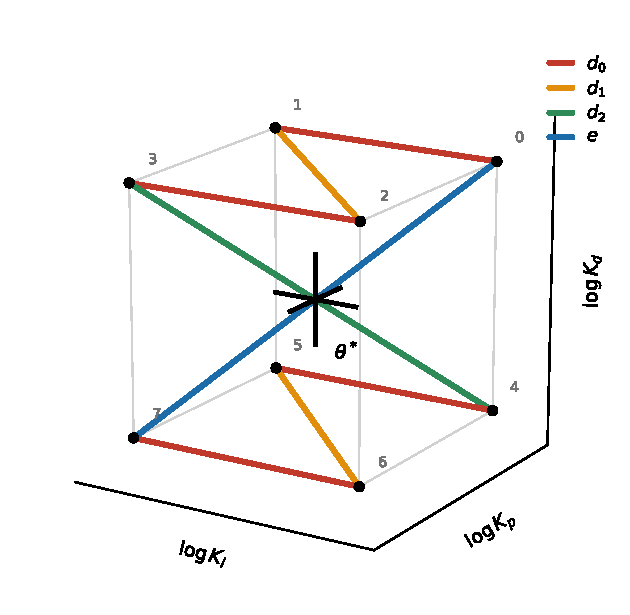
\includegraphics[width=0.9\linewidth]{fig_limit_cycle}
\caption{One period of the terminal orbit in log-gain space, from the move
sequence measured on P1 at $\beta=0.10$ under the regularized index. The eight
points are distinct and the walk closes, as Corollary~\ref{cor:period}
requires; the black cross marks the orbit centre.
% NOTE: redraw from a recorded terminal run if the figure is regenerated.
}
\label{fig:cycle}
\end{figure}

\begin{table}[t]
\small
\centering
\caption{Measured share of the four moves over the last $80$ iterations of a
$400$-iteration run at $\beta = 0.10$ from unit gains, against the prediction
of Proposition~\ref{prop:balance}. Runs use the reference implementation
of \cite{Paper1} with the regularized index \eqref{eq:neps}. Under the
published hard count the same runs miss the prediction by up to $0.04$ and
reach no exactly periodic orbit, which is further evidence for
Section~\ref{sec:index}.}
\label{tab:duty}
\begin{tabular}{lcccc}
\toprule
Plant & $w_e$ & $w_{d_0}$ & $w_{d_1}$ & $w_{d_2}$ \\
\midrule
Predicted & $0.125$ & $0.500$ & $0.250$ & $0.125$ \\
\midrule
P1 & $0.125$ & $0.500$ & $0.250$ & $0.125$ \\
P3 & $0.125$ & $0.500$ & $0.250$ & $0.125$ \\
P4 & $0.113$ & $0.512$ & $0.250$ & $0.125$ \\
\bottomrule
\end{tabular}
\end{table}

\paragraph{Boundary Case} If $\theta^*$ lies outside the gain box, condition
\eqref{eq:triplepoint} cannot be satisfied and the cycle changes character.
The trajectory then settles where, for each band, either the index sits on its
threshold \emph{or} the gain sits on a bound. We call this a complementarity
point. The P2 run of the companion paper is an example. It ends with $K_d$ on
the floor of $0.01$ and indices $N = (0.11,\, 1.04,\, 1.14)$ at gains
$(0.392,\, 0.025,\, 0.01)$. What that paper describes as the rule removing
derivative action on a delay-dominant plant is exactly this boundary case.

% =====================================================================
\section{The Move Table Is Forced}
\label{sec:why}

The results so far describe the cycle produced by one particular table of
moves. It is natural to ask whether that table could have been chosen
differently. It could not. Once the priority order is fixed, the table of
Section~\ref{sec:rule} is the only one possible.

\begin{proposition}[The Move Table is Forced]
\label{prop:unique}
Fix the priority order of the rule. Among move tables in which
(i) every entry lies in $\{-1, 0, +1\}$, so that each gain is multiplied by
$\gamma^{\pm 1}$ or left alone; (ii) $e = (1, \dots, 1)$; and (iii) each
cut $d_k$ decreases its own gain, $d_k[k] = -1$; the staircase table
\eqref{eq:moves} is the \emph{unique} one whose balance weights
\eqref{eq:weights} coincide with the branch frequencies of the priority
logic.
\end{proposition}

\begin{proof}
Counting sign patterns, the priority logic selects $e$ on $1$ of the $2^n$
patterns and $d_k$ on $2^{\,n-k-1}$ of them, so matching requires
$e + \sum_k 2^{\,n-k-1} d_k = 0$. Coordinate $j$ of this reads
$\sum_k 2^{\,n-k-1} d_k[j] = -1$: a signed-binary representation of $-1$ with
digits in $\{-1,0,1\}$. Exactly $n$ such representations exist, indexed by the
position $m$ of the single $-1$ digit, namely $d_m[j] = -1$, $d_k[j] = +1$
for $k > m$ and $0$ for $k < m$. Hypothesis (iii) forces $m = j$, giving
$d_k[j] = +1$ for $j < k$, $-1$ for $j = k$, and $0$ for $j > k$. This is
exactly the table \eqref{eq:moves}.
\end{proof}

Hypotheses (i) and (iii) are both needed: without (iii) there are $n^n$
matching tables, and relaxing (i) to entries in $\{-2, \dots, 2\}$ gives six for
$n = 3$. The triangular shape is therefore not a design choice but the only
shape that fits the selection logic together with the balance condition. The
weights are powers of two because the selection tree is binary.

Two consequences follow. First, the matching gives a useful pairing:
$\lVert d_k \rVert = \sqrt{k+1}$, while $d_k$ occurs with frequency
$2^{-(k+1)}$, so the most frequent move is always the smallest one. Second,
the matching also says something about measurement noise. If noise removes all information from the three signs, the moves occur
at the branch frequencies, and those frequencies are the balance weights. The
expected displacement is then zero, so the iteration stays at $\theta^*$
instead of drifting away. This is a property of the move table and is proved
here by counting. A full stochastic treatment, including the case of
correlated noise where this argument no longer holds, is left to future work.

% =====================================================================
\section{Choosing the Step}
\label{sec:size}

The fixed-step iteration cannot converge to a point, and by
Section~\ref{sec:cycle} it should not be expected to. The practical question is
how far from the target it leaves the gains, and
Corollary~\ref{cor:excursion} answers it without needing the ordering of the
orbit: the excursion is bounded coordinate by coordinate, in units of the step.
Halving $\beta$ therefore halves it exactly.

\begin{corollary}[Design Rule]
\label{cor:design}
On a terminal orbit with $n_e = 1$, the gains stay within the multiplicative
factors
\begin{equation}
K_i : \gamma^{2}, \qquad K_p : \gamma, \qquad K_d : \gamma^{1/2},
\qquad \gamma = (1-\beta)^{-1},
\label{eq:designfwd}
\end{equation}
of their values at the orbit centre, at every iteration. To hold every gain
within a common factor $\rho$ it is therefore enough to choose
\begin{equation}
\boxed{\;\beta \;\le\; 1 - \rho^{-1/2}\;}
\label{eq:designrule}
\end{equation}
\end{corollary}

The bound contains no plant parameter: it comes from the move counts alone.
It is also deliberately asymmetric. The integral gain is moved by all four
moves and the derivative gain by two, so the loosest coordinate is $K_i$ and
the tightest $K_d$. At the companion paper's default $\beta = 0.1$ the
guarantees are $23.5\,\%$ on $K_i$, $11.1\,\%$ on $K_p$ and $5.4\,\%$ on
$K_d$; holding all three within $5\,\%$ requires $\beta \le 0.024$. Where a
run shows $n_e > 1$, as P3 does, the factors compound accordingly.

Three conditions come with \eqref{eq:designrule}. It is exact when the
switching surfaces are locally flat, and curvature adds a term of order $h^2$.
It assumes that $\theta^*$ lies inside the gain box; if it does not, the
boundary case of Section~\ref{sec:cycle} applies. Under measurement noise it
holds down to the noise floor, below which the spread around $\theta^*$ is set
by the noise and not by $\beta$.

It is also worth saying which error is bounded. Equation
\eqref{eq:designrule} bounds the error in the \emph{gains}, and this bound is
the same for every plant. The corresponding error in the turn index is
$|N_k - \Nbar_k| \approx \|J_k\| \, \tfrac{\sqrt{3}}{2} h$, where $J$ is the
local Jacobian of Section~\ref{sec:structure}, and this does depend on the
plant. The indices are the measuring instrument; the gains are the result.

We measure this from far starting points, with the gains detuned by a factor
of $16$. With a constant $\beta$ the run reaches the cycle quickly, and the
final error of $0.074$ is the radius of that cycle. This is a few percent in
each gain, which for
% TODO-REGEN: state beta of this run and compare 0.074 against
% (sqrt(3)/2)*log(gamma) explicitly once the schedule script exists;
% also tabulate the Corollary 3 factor rho for the beta values used.
plant-floor use is indistinguishable from the target. This is the theoretical
support for the companion paper's constant-step recommendation: the fixed-step
rule is guaranteed to leave the gains within one cycle radius of a
plant-determined point, and that radius is set by $\beta$ alone.

% =====================================================================
\section{Local Structure}
\label{sec:structure}

Two facts about the neighborhood of $\theta^*$ shape a proof. The
central-difference Jacobians $\partial N_j/\partial\theta_i$ of the regularized
index are nonsingular on every interior-target plant, with determinants $1.2$,
$5.9$ and $4.3$ on P1, P3, P4, so the center is locally unique. But they are
neither diagonal nor diagonally dominant: on P1 the proportional gain moves the
band-2 index harder than the derivative gain does, and on P4 the own-gain entry
of band~1 is negative. The picture in which each move repairs its own band is
therefore wrong at the center, and a per-move argument fails on two of three
plants --- yet on all three the cycle forms, centers correctly, and shrinks.
% TODO-REGEN: add units/normalization to reproduce script.

The resolution is that the cycle is a property of the \emph{averaged} motion.
Near $\theta^*$ the iteration switches rapidly between the four regions and its
mean motion is the convex combination of their velocities weighted by residence
time, which is the Filippov regularization of the switched system
\cite{Filippov1988}; the measured shares of Table~\ref{tab:duty} are direct
evidence, being exactly the balance weights \eqref{eq:weights}. A proof should
therefore show that $\theta^*$ is a stable equilibrium of the Filippov field
and recover the discrete cycle by averaging. We leave this as the open problem.
Note also that any scheme treating the bands separately, one step size or
momentum term per band, assumes the diagonal structure that is missing here.

\section{The Drift Meter}
\label{sec:detector}\label{sec:accel}

Everything so far describes where the cycle is and how big it is. What the
running rule needs is different: it needs to know \emph{whether it has got
there yet}. This section shows that the balance condition answers that
question too, and that the answer is already contained in the moves the rule
has made, so no extra experiment is required.

The idea is a counting argument. Over a window of recent iterations, count how
often each of the four moves was applied. If the shares match the balance
weights $w$ of \eqref{eq:weights} then by Proposition~\ref{prop:balance} the
moves cancel: the gains have returned where they began and the state is
circling the triple point. If they do not match, the gains are still
travelling --- and the \emph{size} of the mismatch is not a flag but the speed
of travel.

\begin{proposition}[Drift Meter]
\label{prop:meter}
Let $p$ be the vector of observed move shares over any window and $M$ the move
table \eqref{eq:moves}. The mean displacement of the gains per iteration is
\begin{equation}
d \;=\; h\,M^{\!\top} p \;=\; h\,M^{\!\top}(p - w),
\label{eq:meter}
\end{equation}
and its size is fixed by the mismatch $\lVert p-w\rVert$ within a factor
of $1.30$:
\begin{equation}
\sqrt{2}\;h\,\lVert p - w\rVert \;\le\; \lVert d \rVert \;\le\;
1.841\;h\,\lVert p - w\rVert .
\label{eq:meterbound}
\end{equation}
\end{proposition}

\begin{proof}
Each move $v$ is applied a fraction $p_v$ of the time and shifts $\theta$ by
$h\,v$, which is the first equality. The second is $M^{\!\top}w = 0$, that is
\eqref{eq:weights}. Since $p$ and $w$ are both share vectors, $p-w$ sums to
zero; the two constants are the least and greatest singular values of
$M^{\!\top}$ on that subspace, obtained from the move table alone.
\end{proof}

A run climbing reads $\sqrt3\,h$ per iteration, one cutting only the lowest
band reads $1\,h$, one on the cycle reads zero (Fig.~\ref{fig:meter}).

\begin{figure}[t]
\centering
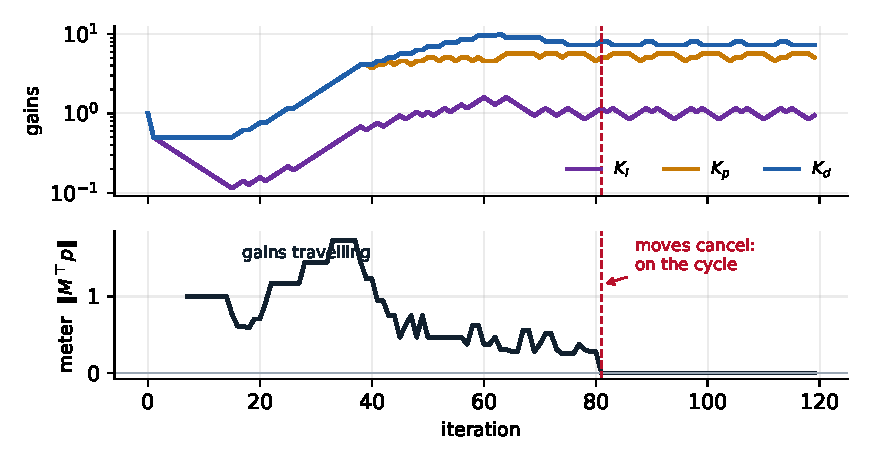
\includegraphics[width=\linewidth]{fig_meter}
\caption{The meter on a run of the published rule (P1, $\beta=0.1$, unit-gain
start). Above, the gains; below, the meter over a sliding window of eight
iterations. While the gains travel it reads of order one; at iteration $81$
the moves begin to cancel and it falls identically to zero, the same instant
the gains stop climbing and begin to cycle. Nothing but the move sequence
enters the lower curve.}
\label{fig:meter}
\end{figure}



Three things make the meter practical. It contains no plant: the constants
come from $M$, which the rule fixes, so they hold for every loop --- unlike
the local Jacobians of Section~\ref{sec:structure}, whose condition numbers
run into the hundreds. Its natural window is the period, since a closed orbit
has counts $n_e(1,4,2,1)$ by Corollary~\ref{cor:period} and eight iterations
therefore read identically zero. And it costs nothing, because the rule
already records which row it fired.

\paragraph{Two uses} \emph{Shrink the step:} while the reading is large the
state is travelling and the step should stay large; once it falls to zero the
step buys no further progress and can be halved, handing the state to a
concentric cycle of half the radius. \emph{Stop tuning:} a zero reading also
means nothing more can be learned by iterating, so the tuner may hold the gains
and stop stepping the plant. Since the reading rises again as soon as the moves
cease to cancel, the same statistic re-arms the tuner if the plant later
drifts, two thresholds giving the hysteresis that avoids chatter.

\paragraph{Why a fixed schedule will not do} A step shrinking with the
iteration number needs no detector, but does not work. From a $16\times$
detuned start the schedules $\beta_n \propto n^{-1/2}$ and $n^{-3/4}$ do reach
$\theta^*$, to $0.010$ and $0.001$, confirming the center; they are analysis
instruments rather than recommendations. The classical $n^{-1}$ stops early at
error $0.197$, for a reason that is a limit on total travel, not noise.

\begin{lemma}[Logarithmic Travel]
\label{lem:travel}
Let $\beta_n = c/n$. The total distance covered in $n$ steps is then
$\sum_{m \le n} \log\gamma_m = -\sum_{m \le n}\log(1 - c/m) = O(\log n)$.
A target at distance $D$ therefore cannot be reached in fewer than about
$n \approx e^{D/c}$ iterations, even if every step points the right way.
\end{lemma}

With $D \approx \log 16$ per gain the required $n$ is enormous --- the same
borderline case as in stochastic approximation, but arising here because the
iteration is deterministic and the path is too short, not because of noise.



\paragraph{Application: a schedule that shrinks only when shrinking helps}
A schedule fixed in advance is either too slow or too weak
as just shown. Proposition~\ref{prop:meter} removes the guesswork.
While $\lVert p - w \rVert$ is large the state is traveling and the step should
stay large; when it falls to the noise floor of the window the state is
orbiting, the step is no longer buying progress, and it can be cut. In the
limiting form of this test one halves $\beta$ once every band has reversed,
which is the cheapest sufficient condition for $p$ to have visited all four
moves. Each halving hands the state from one orbit to a concentric orbit of
half the size, so the error falls geometrically at a bounded number of iterations
per stage. On the interior-target plants this reaches $10^{-4}$ in $36$ to
$98$ iterations, three orders of magnitude better than the constant step for a
comparable number of experiments. This is a global relative of the sign-based Rprop
update with step adaptation on reversal \cite{Riedmiller1993}.

\paragraph{What the meter cannot see} Under noise heavy enough to randomize the
three comparisons, the priority logic fires at its branch frequencies, which by
Proposition~\ref{prop:unique} are the balance weights themselves: the meter
then reads zero although the state is not orbiting, reporting arrival when it
has gone blind. The discriminating feature is the \emph{ordering}, a genuine
orbit being periodic at lag $8$ while noise-driven moves share its marginals in
independent order. A complete detector pairs \eqref{eq:meterbound} with a
periodicity test, left to the stochastic treatment.

% =====================================================================
\section{Conclusions}

SPIN tuning with a fixed step ends in a limit cycle, and that cycle is now
fully described. It circles the triple point, the gain vector fixed by the
plant at which all three turn indices sit on their thresholds. Its move
frequencies $(\tfrac18, \tfrac12, \tfrac14, \tfrac18)$ follow from a single
balance condition, and the same condition over the integers gives the shortest
possible period of $8$. The cycle is realized as a binary counter on the
orbit of period $8$ with counts $(1,4,2,1)$, and those counts alone bound how
far each gain strays from its centre. If the
triple point lies outside the gain box, the cycle instead settles at a
complementarity point, as in the P2 run of the companion paper. Two tools made
the analysis possible: the balance condition, which locates the center, and the
$\varepsilon$-regularized winding index, which makes that center well defined.

The results support practice directly. The excursion bound keeps $K_i$, $K_p$
and $K_d$ within the factors $\gamma^{2}$, $\gamma$, $\gamma^{1/2}$ of their
values at the centre, so a common accuracy $\rho$ follows from
$\beta \le 1-\rho^{-1/2}$. This contains no plant parameter; at the companion
paper's default $\beta = 0.1$ it guarantees $23.5\,\%$, $11.1\,\%$ and
$5.4\,\%$ on the three gains.

The balance condition then closes the circle. Used forwards it locates the
cycle; used backwards it measures the distance to it, since by
Proposition~\ref{prop:meter} the deviation of the observed move frequencies
from the balance weights is the drift rate, to within a factor of $1.30$ and
with constants that involve no plant. The rule can therefore read its own
progress from the sequence of moves it has already made, needing no extra
experiment, and shrink its step only when shrinking it helps: the resulting
schedule reaches $10^{-4}$ accuracy in fewer than a hundred iterations. One
theoretical step remains open, the existence and stability of the cycle
through the averaged Filippov dynamics; and one practical limitation is known,
that the meter cannot distinguish a true orbit from comparisons randomized by
noise, for which the ordering of the moves rather than their frequencies is
the discriminating statistic.

% =====================================================================
\footnotesize
\begin{thebibliography}{10}
\setlength{\itemsep}{-4pt}\setlength{\parsep}{0pt}\setlength{\labelsep}{3pt}
\itemsep0pt

\bibitem{Paper1}
D. Pachner, P. Otta, J. Dost\'al, V. Havlena, Model-free PID tuning by
step-response inspection, submitted to J. Process Control, 2026.

\bibitem{ZN1942}
J.~G. Ziegler, N.~B. Nichols, Optimum settings for automatic controllers,
Trans. ASME 64 (1942) 759--768.

\bibitem{AstromHagglund2004}
K.~J. {\AA}str{\"o}m, T. H{\"a}gglund, Revisiting the Ziegler--Nichols
step response method for PID control, J. Process Control 14 (2004) 635--650.

\bibitem{Hjalmarsson1998}
H. Hjalmarsson, M. Gevers, S. Gunnarsson, O. Lequin, Iterative feedback
tuning: theory and applications, IEEE Control Syst. Mag. 18 (4) (1998)
26--41.

\bibitem{Killingsworth2006}
N.~J. Killingsworth, M. Krsti{\'c}, PID tuning using extremum seeking,
IEEE Control Syst. Mag. 26 (1) (2006) 70--79.

\bibitem{Riedmiller1993}
M. Riedmiller, H. Braun, A direct adaptive method for faster backpropagation
learning: the RPROP algorithm, in: Proc. IEEE Int. Conf. Neural Networks,
1993, pp. 586--591.

\bibitem{Filippov1988}
A.~F. Filippov, Differential Equations with Discontinuous Righthand Sides,
Kluwer, 1988.

\end{thebibliography}

\end{document}
